\subsubsubsection{Brisanje naloga snabdevača}

\begin{itemize}
    \item Kratak opis:
        \begin{itemize}
            \item Administrator vrši raskid ugovora sa snabdevačem i briše njegov nalog.
        \end{itemize}
    \item Učesnici:
        \begin{itemize}
            \item Administrator
            \item Snabdevač
        \end{itemize}
    \item Preduslovi:
        \begin{itemize}
            \item Snabdevač je registrovan i prekršio je neku od klauzula ugovora.
            \item Snabdevač je prijavljen i želi da obriše svoj nalog.
            
            
        \end{itemize}
    \item Postuslovi:
        \begin{itemize}
            \item Uspešno je raskinut ugovor između snabdevača i HelloFresh kompanije.
            \item Snabdevač prestaje se uslugom dostavljanja namirnica.
            \item Nalog snabdevača je obrisan iz sistema.
        \end{itemize}
    \item Osnovni tok:
         \begin{enumerate}
            \item Administrator uočava da je snabdevač prekršio uslove ugovora.
            \item Administrator vrši raskid ugovora i obaveštava snabdevača o raskidu.
            \item Administrator bira opciju za brisanje naloga snabdevača.
            \item Sistem uklanja snabdevača iz spiska dostupnih snabdevača i briše njegov nalog.
        \end{enumerate}
    \item Alternativni tok:
        \begin{itemize}
            \item[1.a] Snabdevač putem veb stranice podnosi zahtev za brisanje naloga. Slučaj upotrebe se nastavlja od koraka 2.
        \end{itemize}
\end{itemize}

\begin{figure}[H]
\begin{center}
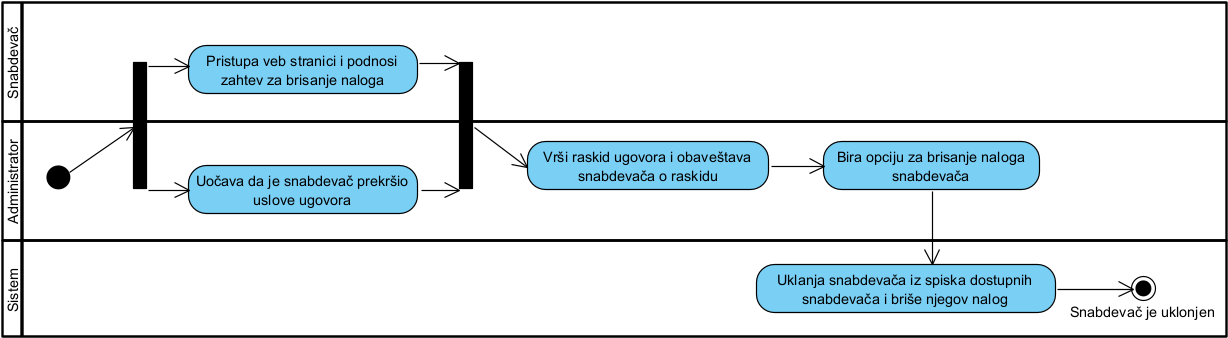
\includegraphics[width=\textwidth]{Pictures/activity_supplier_delete.png}
\end{center}
    \caption{Dijagram aktivnosti brisanja naloga snabdevača}
\label{fig:ActivitySupplierContractTermination1}
\end{figure}